\documentclass{beamer}
%\documentclass[handout]{beamer}
%\usepackage{pgfpages}
%\pgfpagesuselayout{2 on 1}[a4paper,border shrink=5mm]

\usepackage{verbatim}
\usepackage{amssymb}
\usepackage{amsmath}

\mode<presentation>
{
  \usetheme{Singapore}  %Warsaw}  %CambridgeUS}
  
  \setbeamercovered{transparent}
  }


\usepackage[english]{babel}
\usepackage[latin1]{inputenc}
\usepackage{times}
\usepackage[T1]{fontenc}
\newcommand{\bs}{\boldsymbol}
\newcommand{\mb}{\mathbf}
\newcommand{\x}{\mathbf{x}}
\newcommand{\X}{\mathbf{X}}
\newcommand{\y}{\mathbf{y}}
\newcommand{\Y}{\mathbf{Y}}

\title[Flexible Bivariate Regression] {Flexible Bivariate Regression}

%\subtitle
%{Descriptive Questions} 

%\author[Adam Glynn]{Adam Glynn}
%\institute[Harvard University]{Harvard University} 

\date{September 1, 2022}

\subject{Talks}

\AtBeginSection[]
{
  \begin{frame}<beamer>
    \frametitle{Outline}
    \tableofcontents[currentsection,currentsubsection]
  \end{frame}
}


\AtBeginSubsection[]
{
  \begin{frame}<beamer>
    \frametitle{Outline}
    \tableofcontents[currentsection,currentsubsection]
  \end{frame}
}

\begin{document}

\begin{frame}
  \titlepage
\end{frame}




\begin{frame}
  \frametitle{Outline}
  \tableofcontents
 
\end{frame}





\section{Flexibility with ``Linear'' Regression}



\frame{
\frametitle{Nonlinear ``Linear'' Regression}

\begin{itemize}
\item Fitted Values from the LCMF $\hat{y}_i = B_0 + B_1 x_i + B_2 x_i^2$\\
 for $i=1,...,N$ \pause
\item Residuals from Fitted Values:  $e_i = y_i - \hat{y}_i$ for $i=1,...,N$
\end{itemize} \pause

\vspace{.5cm}

Again, we choose $B_0$, $B_1$, and $B_2$, to minimize the SSR, where
\begin{align*}
SSR &= \sum_{i=1}^N e_i^2
\end{align*}
but the definition of $e_i$ changes with the inclusion of polynomial terms. 
}


\frame{
\frametitle{Recall: Simple Regression with SCscore}

$$\widehat{CLlib}_i = B_0 + B_1 \cdot SCscore_i $$

\begin{figure}[ht] \centering
        \scalebox{.4}{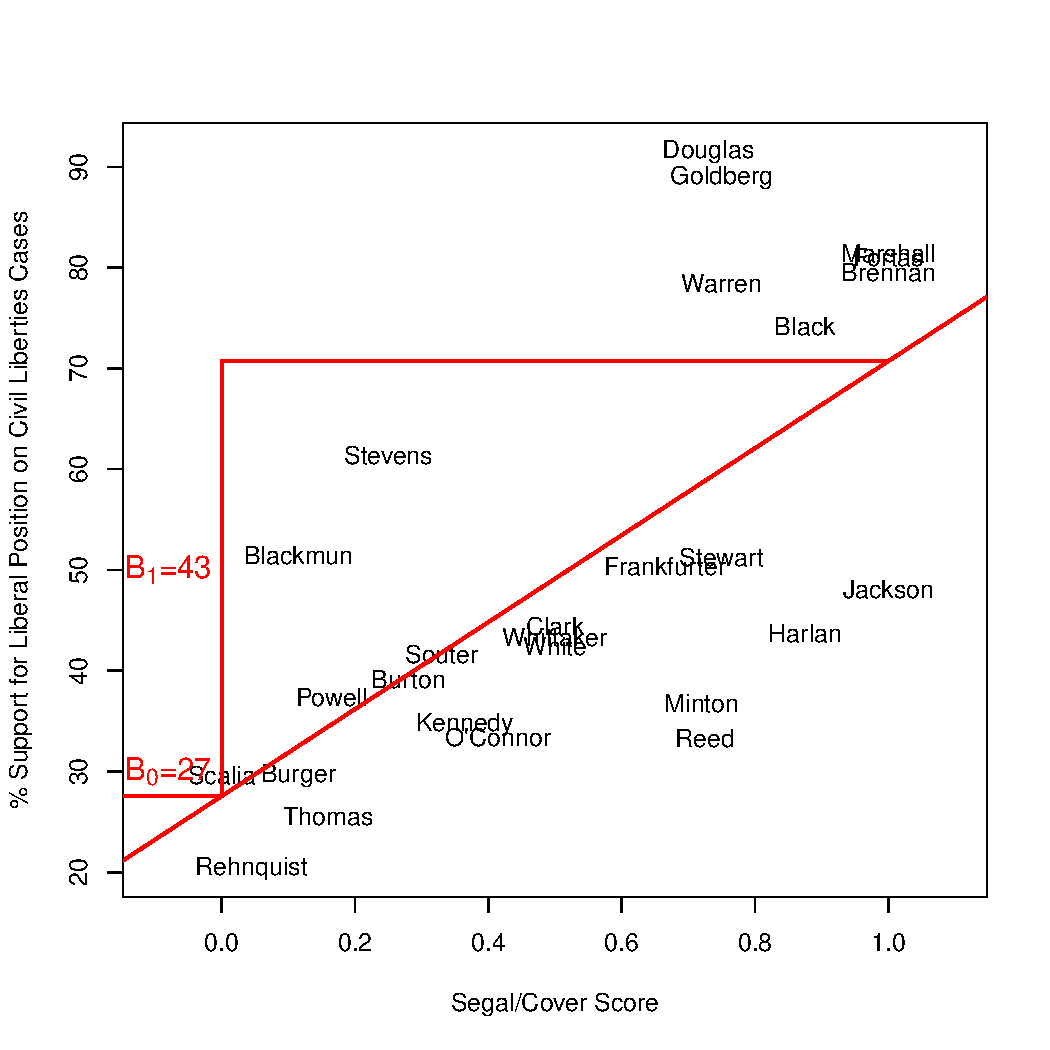
\includegraphics{lmPlot.pdf}}
\end{figure}

}

\frame{
\frametitle{Quadratic Regression with SCscore}

$$\widehat{CLlib}_i = B_0 + B_1 \cdot SCscore_i  + B_2 \cdot SCscore_i^2$$

\begin{figure}[ht] \centering
        \scalebox{.4}{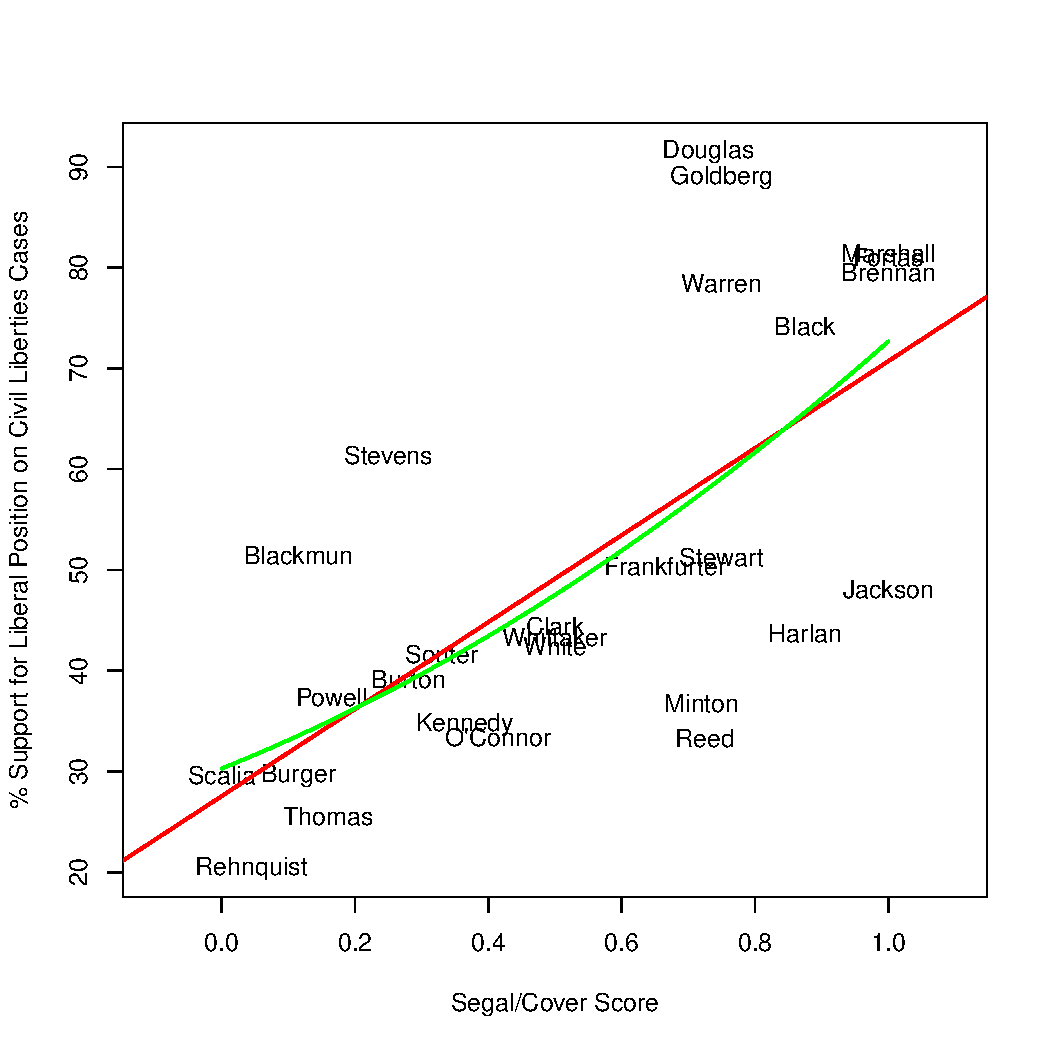
\includegraphics{QuadLmPlot.pdf}}
\end{figure}

}



\section{Flexibility with ML approaches}



\frame{
\frametitle{Loess with SCscore}

$$\widehat{CLlib}_i = f(SCscore_i)$$

\begin{figure}[ht] \centering
        \scalebox{.4}{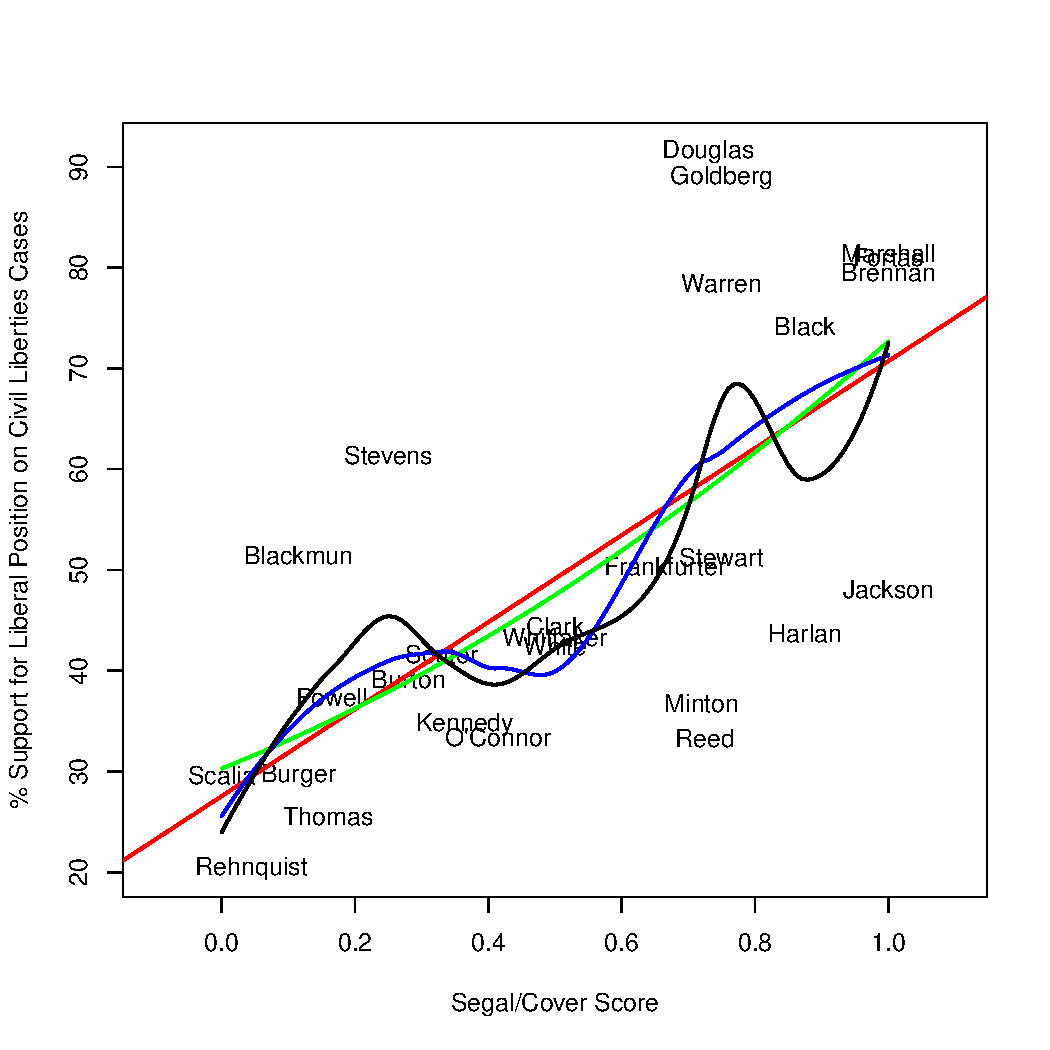
\includegraphics{LoessPlot.pdf}}
\end{figure}

}

\frame{
\frame{Summary and transition to board work}

\begin{itemize}
\item We can increase flexibility within ``linear'' regression by adding polynomial terms.
\item ML techniques like splines and kernel methods (e.g., loess) provide a better option
\item On the board.... We can choose flexibility with LOOCV.  
\end{itemize}

}

\end{document}












